\documentclass{beamer}
\usepackage{geometry}
\usepackage[utf8]{inputenc}
\usepackage{microtype}
\usepackage{amsmath}
\usepackage{amssymb}
\usepackage{siunitx} %units in math. eg 20\milli\meter
\usepackage{yhmath} % for arcs, overparenth command
\usepackage{tikz} %graphics
\usetikzlibrary{quotes, angles}
\usepackage{graphicx} %consider setting \graphicspath
%\usepackage{enumitem} incompatible with beamer class
\usepackage{multicol}
\usepackage{venndiagram}


\setlength{\headheight}{26pt}%doesn't seem to fix warning

\usepackage{fancyhdr}
\pagestyle{fancy}
\fancyhf{}

%\rhead{\small{13 September 2021}}
\lhead{\small{BECA / Dr. Huson / Geometry Unit 2}}

\renewcommand{\headrulewidth}{0pt}

\title{Mathematics Class Slides}
\subtitle{Bronx Early College Academy}
\author{Christopher J. Huson PhD}
\date{28 September - 7 October 2022}

\begin{document}
\frame{\titlepage}
\section[Outline]{}
\frame{\tableofcontents}

\section{2.1 Angles and their measures, 28 September}
\frame
{
  \frametitle{Learning Target: I can measure angles}
  \framesubtitle{CCSS: HSG.CO.A.1 Know precise geometric definitions  \hfill \alert{2.1 Monday 28 Sept}}

  \begin{block}{Do Now: On the clock face, which is more time, from the 1 to the 3, or from the 11 to the 2? (insert clock image)}
    \begin{tikzpicture}
      \draw [->, thick] (0,0)--(-1,2);
      \draw (0,0) circle [radius=2];
    \end{tikzpicture} 
  \begin{enumerate}
    \item Write down an equation to represent the situation.
  \end{enumerate}
  \end{block}
  Lesson: Angle measures, internal, external, acute, obtuse, right
}

\frame
{
  \frametitle{Angle: two rays with a common endpoint or vertex}
  Rays $\overrightarrow{BA}$ and $\overrightarrow{BC}$. Vertex $B$.
  Written notation is $\angle ABC$ or $\angle B$. \\[0.75cm]
        \begin{center}
          \begin{tikzpicture}
            \draw [<->, thick] (45:6)--(0,0)--(6,0);
            \draw [fill] (45:4) circle [radius=0.05] node[below]{$A$};
            \draw [fill] (0,0) circle [radius=0.05] node[below]{$B$};
            \draw [fill] (4,0) circle [radius=0.05] node[below]{$C$};
          \end{tikzpicture}
          \end{center}
}

\frame
{
  \frametitle{Angle measures: the Babylonian system of $360^\circ$ in a circle}
    \begin{itemize}
      \item A full rotation is $360^\circ$ (a full ``turn'').
      \item A half turn (straight line) is $180^\circ$.
      \item $90^\circ$ is a quarter turn or a \emph{right} angle.
      \item \emph{Acute} angles measure less than $90^\circ$. \emph{Obtuse} angles measure more than $90^\circ$.
      \item \emph{Adjacent} angles (``next to'' each other) share a common ray and are external to each other.
    \end{itemize}
  \begin{center}
    \begin{tikzpicture}
      \draw [<->, thick] (25:6)--(0,0)--(6,0);
      \draw [->, thick] (0,0)--(75:3);
      \draw [fill] (0,0) circle [radius=0.05] node[below]{$A$};
      %\draw [fill] (7,0) circle [radius=0.05] node[below]{$N$};
    \end{tikzpicture}
    \end{center}
}

\section{2.2 Angle addition, 29 September}
\frame
{
  \frametitle{Learning Target: I can solve for angle measures}
  \framesubtitle{CCSS: HSG.CO.A.1 Know precise geometric definitions  \hfill \alert{2.2 Tuesday 29 Sept}}

  \begin{block}{Do Now: $m\angle ABD=30^\circ$, $m\angle DBC=45^\circ$. Find $m\angle ABC$.}\vspace{0.5cm}
          \begin{center}
            \begin{tikzpicture}
              \draw [<->, thick] (45:5)--(0,0)--(6,0);
              \draw [->, thick] (0,0)--(75:4);
              \draw [fill] (75:3) circle [radius=0.05] node[left]{$A$};
              \draw [fill] (45:3) circle [radius=0.05] node[below right]{$D$};
              \draw [fill] (0,0) circle [radius=0.05] node[below]{$B$};
              \draw [fill] (4,0) circle [radius=0.05] node[below]{$C$};
              \node at (1.5,0.5){$45^\circ$};
              \node at (1,1.7){$30^\circ$};
            \end{tikzpicture}
            \end{center}
  \end{block}
  Lesson: Angle addition problems, vertical angles
}

\frame
  {
    \frametitle{Angle addition postulate}

    For adjacent angles, the sum of their measures is the measure of their combined angle.\\
    Special pairs of angles [make a new slide]\\
    A \emph{linear pair} are two angles that make a straight line. \\
    \emph{Opposite rays} have a common endpoint and make a line. (They form an angle measuring $180^\circ$).\\
    Angles whose measures sum to $180^\circ$ are \emph{supplementary}. \\
    Angles whose measures sum to $90^\circ$ are \emph{complementary}.
    \begin{center}
      \begin{tikzpicture}
        \draw [<->, thick] (45:3)--(0,0)--(4,0);
        \draw [->, thick] (0,0)--(125:2);
        \draw [fill] (0,0) circle [radius=0.05] node[below]{$A$};
        %\draw [fill] (7,0) circle [radius=0.05] node[below]{$N$};
      \end{tikzpicture}
      \end{center}
  }

\section{2.3 Angle bisectors, 30 September}
\frame
{
  \frametitle{Learning Target: I can bisect angles}
  \framesubtitle{CCSS: HSG.CO.A.1 Know precise geometric definitions  \hfill \alert{2.3 Friday 30 Sept}}

  Definition of angle bisector\\
  \emph{Angle bisector:} a ray dividing an angle into two congruent angles.\\[0.5cm]
  As shown, $\overrightarrow{BD}$ bisects $\angle ABC$ if and only if $\angle ABD \cong \angle CBD$. 
  \begin{center}
    \begin{tikzpicture}
      \draw [<->, thick] (40:4)--(0,0)--(4,0);
      \draw [->, thick] (0,0)--(80:3);
      \draw [fill] (40:3) circle [radius=0.05] node[below right]{$D$};
      \draw [fill] (80:2) circle [radius=0.05] node[left]{$A$};
      \draw [fill] (0,0) circle [radius=0.05] node[below]{$B$};
      \draw [fill] (3,0) circle [radius=0.05] node[below]{$C$};
    \end{tikzpicture}
    \end{center}
}

\section{2.4 Vertical angles, 2 October}
\frame
{
  \frametitle{Learning Target: I can identify vertical angles}
  \framesubtitle{CCSS: HSG.CO.A.1 Know precise geometric definitions  \hfill \alert{2.4 Friday 2 October}}

  Definition: \emph{Vertical angles} are angles opposite each other when two lines intersect. $\angle 1$ and $\angle 3$ are vertical angles, as are $\angle 2$ and $\angle 4$.
\begin{center}
\begin{tikzpicture}[scale=0.5, rotate=15]
  \draw [<->, thick] (0,-1.5)--(10,1.5);
  \draw [<->, thick] (2,3.5)--(7,-3.5);
  \node at (3,.4){1};
  \node at (6,-.6){3};
  \node at (5,1){2};
  \node at (4,-1){4};
  %\draw [fill] (0,0) circle [radius=0.05] node[below]{$P$};
  %\draw [fill] (6,0) circle [radius=0.05] node[below]{$R$};
  %\draw [fill] (3,0) circle [radius=0.05] node[below]{$Q$};
\end{tikzpicture}
\end{center}
  Lesson: Angle addition problems, vertical angles
}

\section{Open Middle: complementary and supplementary puzzle}
\frame
{
  \frametitle{Open Middle problem (fun) \\
  Use digits from 0 to 9. Using a digit no more than once.}
    The first two angle measures are complementary. The second two angles supplementary. (degrees)\\[0.75cm]
      \begin{tikzpicture}
        \draw (0,0) rectangle (1,1);
        \draw (1.25,0) rectangle (2.25,1);
        \draw (3.25,0) rectangle (4.25,1);
        \draw (4.5,0) rectangle (5.5,1);

        \draw (-1.25,-1.5) rectangle (-0.25,-0.5);
        \draw (0,-1.5) rectangle (1,-0.5);
        \draw (1.25,-1.5) rectangle (2.25,-0.5);
        \draw (3.25,-1.5) rectangle (4.25,-0.5);
        \draw (4.5,-1.5) rectangle (5.5,-0.5);
      \end{tikzpicture} \vspace{5cm} 
}

\end{document}